\documentclass[twoside]{book}

% Packages required by doxygen
\usepackage{fixltx2e}
\usepackage{calc}
\usepackage{doxygen}
\usepackage[export]{adjustbox} % also loads graphicx
\usepackage{graphicx}
\usepackage[utf8]{inputenc}
\usepackage{makeidx}
\usepackage{multicol}
\usepackage{multirow}
\PassOptionsToPackage{warn}{textcomp}
\usepackage{textcomp}
\usepackage[nointegrals]{wasysym}
\usepackage[table]{xcolor}

% Font selection
\usepackage[T1]{fontenc}
\usepackage[scaled=.90]{helvet}
\usepackage{courier}
\usepackage{amssymb}
\usepackage{sectsty}
\renewcommand{\familydefault}{\sfdefault}
\allsectionsfont{%
  \fontseries{bc}\selectfont%
  \color{darkgray}%
}
\renewcommand{\DoxyLabelFont}{%
  \fontseries{bc}\selectfont%
  \color{darkgray}%
}
\newcommand{\+}{\discretionary{\mbox{\scriptsize$\hookleftarrow$}}{}{}}

% Page & text layout
\usepackage{geometry}
\geometry{%
  a4paper,%
  top=2.5cm,%
  bottom=2.5cm,%
  left=2.5cm,%
  right=2.5cm%
}
\tolerance=750
\hfuzz=15pt
\hbadness=750
\setlength{\emergencystretch}{15pt}
\setlength{\parindent}{0cm}
\setlength{\parskip}{3ex plus 2ex minus 2ex}
\makeatletter
\renewcommand{\paragraph}{%
  \@startsection{paragraph}{4}{0ex}{-1.0ex}{1.0ex}{%
    \normalfont\normalsize\bfseries\SS@parafont%
  }%
}
\renewcommand{\subparagraph}{%
  \@startsection{subparagraph}{5}{0ex}{-1.0ex}{1.0ex}{%
    \normalfont\normalsize\bfseries\SS@subparafont%
  }%
}
\makeatother

% Headers & footers
\usepackage{fancyhdr}
\pagestyle{fancyplain}
\fancyhead[LE]{\fancyplain{}{\bfseries\thepage}}
\fancyhead[CE]{\fancyplain{}{}}
\fancyhead[RE]{\fancyplain{}{\bfseries\leftmark}}
\fancyhead[LO]{\fancyplain{}{\bfseries\rightmark}}
\fancyhead[CO]{\fancyplain{}{}}
\fancyhead[RO]{\fancyplain{}{\bfseries\thepage}}
\fancyfoot[LE]{\fancyplain{}{}}
\fancyfoot[CE]{\fancyplain{}{}}
\fancyfoot[RE]{\fancyplain{}{\bfseries\scriptsize Generated by Doxygen }}
\fancyfoot[LO]{\fancyplain{}{\bfseries\scriptsize Generated by Doxygen }}
\fancyfoot[CO]{\fancyplain{}{}}
\fancyfoot[RO]{\fancyplain{}{}}
\renewcommand{\footrulewidth}{0.4pt}
\renewcommand{\chaptermark}[1]{%
  \markboth{#1}{}%
}
\renewcommand{\sectionmark}[1]{%
  \markright{\thesection\ #1}%
}

% Indices & bibliography
\usepackage{natbib}
\usepackage[titles]{tocloft}
\setcounter{tocdepth}{3}
\setcounter{secnumdepth}{5}
\makeindex

% Hyperlinks (required, but should be loaded last)
\usepackage{ifpdf}
\ifpdf
  \usepackage[pdftex,pagebackref=true]{hyperref}
\else
  \usepackage[ps2pdf,pagebackref=true]{hyperref}
\fi
\hypersetup{%
  colorlinks=true,%
  linkcolor=blue,%
  citecolor=blue,%
  unicode%
}

% Custom commands
\newcommand{\clearemptydoublepage}{%
  \newpage{\pagestyle{empty}\cleardoublepage}%
}

\usepackage{caption}
\captionsetup{labelsep=space,justification=centering,font={bf},singlelinecheck=off,skip=4pt,position=top}

%===== C O N T E N T S =====

\begin{document}

% Titlepage & ToC
\hypersetup{pageanchor=false,
             bookmarksnumbered=true,
             pdfencoding=unicode
            }
\pagenumbering{alph}
\begin{titlepage}
\vspace*{7cm}
\begin{center}%
{\Large My Project }\\
\vspace*{1cm}
{\large Generated by Doxygen 1.8.14}\\
\end{center}
\end{titlepage}
\clearemptydoublepage
\pagenumbering{roman}
\tableofcontents
\clearemptydoublepage
\pagenumbering{arabic}
\hypersetup{pageanchor=true}

%--- Begin generated contents ---
\chapter{I\+P\+A\+SS pong project}
\label{index}\hypertarget{index}{}\begin{DoxyAuthor}{Author}
Thomas Theil 
\end{DoxyAuthor}
\begin{DoxyDate}{Date}
25-\/06-\/2018 14\+:00 
\end{DoxyDate}

\chapter{Hierarchical Index}
\section{Class Hierarchy}
This inheritance list is sorted roughly, but not completely, alphabetically\+:\begin{DoxyCompactList}
\item \contentsline{section}{c\+Ball}{\pageref{classc_ball}}{}
\item \contentsline{section}{controler}{\pageref{classcontroler}}{}
\begin{DoxyCompactList}
\item \contentsline{section}{G\+Y61}{\pageref{class_g_y61}}{}
\item \contentsline{section}{H\+C\+S\+R04}{\pageref{class_h_c_s_r04}}{}
\item \contentsline{section}{potmeter}{\pageref{classpotmeter}}{}
\item \contentsline{section}{tiny\+Lider}{\pageref{classtiny_lider}}{}
\item \contentsline{section}{Y\+L40}{\pageref{class_y_l40}}{}
\end{DoxyCompactList}
\item \contentsline{section}{c\+Paddel}{\pageref{classc_paddel}}{}
\item \contentsline{section}{piezo}{\pageref{classpiezo}}{}
\item \contentsline{section}{pong\+Manger}{\pageref{classpong_manger}}{}
\end{DoxyCompactList}

\chapter{Class Index}
\section{Class List}
Here are the classes, structs, unions and interfaces with brief descriptions\+:\begin{DoxyCompactList}
\item\contentsline{section}{\mbox{\hyperlink{classc_ball}{c\+Ball}} }{\pageref{classc_ball}}{}
\item\contentsline{section}{\mbox{\hyperlink{classcontroler}{controler}} }{\pageref{classcontroler}}{}
\item\contentsline{section}{\mbox{\hyperlink{classc_paddel}{c\+Paddel}} }{\pageref{classc_paddel}}{}
\item\contentsline{section}{\mbox{\hyperlink{class_g_y61}{G\+Y61}} }{\pageref{class_g_y61}}{}
\item\contentsline{section}{\mbox{\hyperlink{class_h_c_s_r04}{H\+C\+S\+R04}} }{\pageref{class_h_c_s_r04}}{}
\item\contentsline{section}{\mbox{\hyperlink{classpiezo}{piezo}} }{\pageref{classpiezo}}{}
\item\contentsline{section}{\mbox{\hyperlink{classpong_manger}{pong\+Manger}} }{\pageref{classpong_manger}}{}
\item\contentsline{section}{\mbox{\hyperlink{classpotmeter}{potmeter}} }{\pageref{classpotmeter}}{}
\item\contentsline{section}{\mbox{\hyperlink{classtiny_lider}{tiny\+Lider}} }{\pageref{classtiny_lider}}{}
\item\contentsline{section}{\mbox{\hyperlink{class_y_l40}{Y\+L40}} }{\pageref{class_y_l40}}{}
\end{DoxyCompactList}

\chapter{Class Documentation}
\hypertarget{classc_ball}{}\section{c\+Ball Class Reference}
\label{classc_ball}\index{c\+Ball@{c\+Ball}}
\subsection*{Public Member Functions}
\begin{DoxyCompactItemize}
\item 
\mbox{\hyperlink{classc_ball_a26865bcbfe3d50d5e938ec29eec791dd}{c\+Ball}} (int posX, int posY)
\begin{DoxyCompactList}\small\item\em \mbox{\hyperlink{classc_ball}{c\+Ball}} \end{DoxyCompactList}\item 
void \mbox{\hyperlink{classc_ball_a7c7b2cda898f6e1670faa2f753b9c420}{Reset}} ()
\begin{DoxyCompactList}\small\item\em \mbox{\hyperlink{classc_ball_a7c7b2cda898f6e1670faa2f753b9c420}{Reset()}} \end{DoxyCompactList}\item 
void \mbox{\hyperlink{classc_ball_a34a6133cf86c6a333ae9b14eef4d3f99}{change\+Dir}} (int new\+Dir)
\begin{DoxyCompactList}\small\item\em \mbox{\hyperlink{classc_ball_a34a6133cf86c6a333ae9b14eef4d3f99}{change\+Dir()}} \end{DoxyCompactList}\item 
void \mbox{\hyperlink{classc_ball_a65fd252361fa42fbe843a3cc73f2ebdb}{ramdomdir}} (char treshold\+Left=3, char treshold\+Right=1)
\begin{DoxyCompactList}\small\item\em ramdomdir(char tresholdleft, treshold\+Right) \end{DoxyCompactList}\item 
void \mbox{\hyperlink{classc_ball_acbdd0fa42ab6efd934d4966f3bf2e411}{update}} ()
\begin{DoxyCompactList}\small\item\em \mbox{\hyperlink{classc_ball_acbdd0fa42ab6efd934d4966f3bf2e411}{update()}} \end{DoxyCompactList}\item 
int \mbox{\hyperlink{classc_ball_a6216240ba8780e2510c2d2eb5c792be0}{getX}} ()
\begin{DoxyCompactList}\small\item\em int \mbox{\hyperlink{classc_ball_a6216240ba8780e2510c2d2eb5c792be0}{get\+X()}} \end{DoxyCompactList}\item 
int \mbox{\hyperlink{classc_ball_a4439db1ba25e8f69fde4fdf0fa1b4f24}{getY}} ()
\begin{DoxyCompactList}\small\item\em int \mbox{\hyperlink{classc_ball_a4439db1ba25e8f69fde4fdf0fa1b4f24}{get\+Y()}} \end{DoxyCompactList}\item 
int \mbox{\hyperlink{classc_ball_aabb4c1b801ca98f18461f0abebd22e41}{get\+Dir}} ()
\begin{DoxyCompactList}\small\item\em int \mbox{\hyperlink{classc_ball_a4439db1ba25e8f69fde4fdf0fa1b4f24}{get\+Y()}} \end{DoxyCompactList}\end{DoxyCompactItemize}


\subsection{Constructor \& Destructor Documentation}
\mbox{\Hypertarget{classc_ball_a26865bcbfe3d50d5e938ec29eec791dd}\label{classc_ball_a26865bcbfe3d50d5e938ec29eec791dd}} 
\index{c\+Ball@{c\+Ball}!c\+Ball@{c\+Ball}}
\index{c\+Ball@{c\+Ball}!c\+Ball@{c\+Ball}}
\subsubsection{\texorpdfstring{c\+Ball()}{cBall()}}
{\footnotesize\ttfamily c\+Ball\+::c\+Ball (\begin{DoxyParamCaption}\item[{int}]{posX,  }\item[{int}]{posY }\end{DoxyParamCaption})}



\mbox{\hyperlink{classc_ball}{c\+Ball}} 

\begin{DoxyAuthor}{Author}
Thomas Theil 
\end{DoxyAuthor}
\begin{DoxyDate}{Date}
25-\/06-\/2018 15\+:00
\end{DoxyDate}
This class controlles a ball of the game pong

\mbox{\hyperlink{classc_ball}{c\+Ball}} initialize(example) 
\begin{DoxyCode}
\mbox{\hyperlink{classc_ball}{cBall}} ball(x,y);
\end{DoxyCode}
 

\subsection{Member Function Documentation}
\mbox{\Hypertarget{classc_ball_a34a6133cf86c6a333ae9b14eef4d3f99}\label{classc_ball_a34a6133cf86c6a333ae9b14eef4d3f99}} 
\index{c\+Ball@{c\+Ball}!change\+Dir@{change\+Dir}}
\index{change\+Dir@{change\+Dir}!c\+Ball@{c\+Ball}}
\subsubsection{\texorpdfstring{change\+Dir()}{changeDir()}}
{\footnotesize\ttfamily void c\+Ball\+::change\+Dir (\begin{DoxyParamCaption}\item[{int}]{new\+Dir }\end{DoxyParamCaption})}



\mbox{\hyperlink{classc_ball_a34a6133cf86c6a333ae9b14eef4d3f99}{change\+Dir()}} 

changing the directon of the ball

\begin{DoxyParagraph}{Posible directions}
{\bfseries 0} stop ~\newline
 {\bfseries 1} left ~\newline
 {\bfseries 2} upleft ~\newline
 {\bfseries 3} downleft ~\newline
 {\bfseries 4} right ~\newline
 {\bfseries 5} upright ~\newline
 {\bfseries 6} downright ~\newline
 
\end{DoxyParagraph}
\mbox{\Hypertarget{classc_ball_aabb4c1b801ca98f18461f0abebd22e41}\label{classc_ball_aabb4c1b801ca98f18461f0abebd22e41}} 
\index{c\+Ball@{c\+Ball}!get\+Dir@{get\+Dir}}
\index{get\+Dir@{get\+Dir}!c\+Ball@{c\+Ball}}
\subsubsection{\texorpdfstring{get\+Dir()}{getDir()}}
{\footnotesize\ttfamily int c\+Ball\+::get\+Dir (\begin{DoxyParamCaption}{ }\end{DoxyParamCaption})}



int \mbox{\hyperlink{classc_ball_a4439db1ba25e8f69fde4fdf0fa1b4f24}{get\+Y()}} 

get the ball direction for with the ball is traveling in ~\newline
see \mbox{\hyperlink{classc_ball_a34a6133cf86c6a333ae9b14eef4d3f99}{change\+Dir()}} for the meaning of the directions.

\begin{DoxyReturn}{Returns}
int 
\end{DoxyReturn}
\mbox{\Hypertarget{classc_ball_a6216240ba8780e2510c2d2eb5c792be0}\label{classc_ball_a6216240ba8780e2510c2d2eb5c792be0}} 
\index{c\+Ball@{c\+Ball}!getX@{getX}}
\index{getX@{getX}!c\+Ball@{c\+Ball}}
\subsubsection{\texorpdfstring{get\+X()}{getX()}}
{\footnotesize\ttfamily int c\+Ball\+::getX (\begin{DoxyParamCaption}{ }\end{DoxyParamCaption})}



int \mbox{\hyperlink{classc_ball_a6216240ba8780e2510c2d2eb5c792be0}{get\+X()}} 

get the ball it X axis

\begin{DoxyReturn}{Returns}
int 
\end{DoxyReturn}
\mbox{\Hypertarget{classc_ball_a4439db1ba25e8f69fde4fdf0fa1b4f24}\label{classc_ball_a4439db1ba25e8f69fde4fdf0fa1b4f24}} 
\index{c\+Ball@{c\+Ball}!getY@{getY}}
\index{getY@{getY}!c\+Ball@{c\+Ball}}
\subsubsection{\texorpdfstring{get\+Y()}{getY()}}
{\footnotesize\ttfamily int c\+Ball\+::getY (\begin{DoxyParamCaption}{ }\end{DoxyParamCaption})}



int \mbox{\hyperlink{classc_ball_a4439db1ba25e8f69fde4fdf0fa1b4f24}{get\+Y()}} 

get the ball it Y axis

\begin{DoxyReturn}{Returns}
int 
\end{DoxyReturn}
\mbox{\Hypertarget{classc_ball_a65fd252361fa42fbe843a3cc73f2ebdb}\label{classc_ball_a65fd252361fa42fbe843a3cc73f2ebdb}} 
\index{c\+Ball@{c\+Ball}!ramdomdir@{ramdomdir}}
\index{ramdomdir@{ramdomdir}!c\+Ball@{c\+Ball}}
\subsubsection{\texorpdfstring{ramdomdir()}{ramdomdir()}}
{\footnotesize\ttfamily void c\+Ball\+::ramdomdir (\begin{DoxyParamCaption}\item[{char}]{treshold\+Left = {\ttfamily 3},  }\item[{char}]{treshold\+Right = {\ttfamily 1} }\end{DoxyParamCaption})}



ramdomdir(char tresholdleft, treshold\+Right) 

changing to a ramdom direction left or right. 1 a ramdom direction to the left 2 a ramdom direction to the right

\begin{DoxyParagraph}{example}

\begin{DoxyCode}
ball.ramdomdir(\textcolor{keywordtype}{char} dir);
\end{DoxyCode}
 
\end{DoxyParagraph}
\mbox{\Hypertarget{classc_ball_a7c7b2cda898f6e1670faa2f753b9c420}\label{classc_ball_a7c7b2cda898f6e1670faa2f753b9c420}} 
\index{c\+Ball@{c\+Ball}!Reset@{Reset}}
\index{Reset@{Reset}!c\+Ball@{c\+Ball}}
\subsubsection{\texorpdfstring{Reset()}{Reset()}}
{\footnotesize\ttfamily void c\+Ball\+::\+Reset (\begin{DoxyParamCaption}{ }\end{DoxyParamCaption})}



\mbox{\hyperlink{classc_ball_a7c7b2cda898f6e1670faa2f753b9c420}{Reset()}} 

It will reset the ball to its starting position

(example) 
\begin{DoxyCode}
ball.Reset();
\end{DoxyCode}
 \mbox{\Hypertarget{classc_ball_acbdd0fa42ab6efd934d4966f3bf2e411}\label{classc_ball_acbdd0fa42ab6efd934d4966f3bf2e411}} 
\index{c\+Ball@{c\+Ball}!update@{update}}
\index{update@{update}!c\+Ball@{c\+Ball}}
\subsubsection{\texorpdfstring{update()}{update()}}
{\footnotesize\ttfamily void c\+Ball\+::update (\begin{DoxyParamCaption}{ }\end{DoxyParamCaption})}



\mbox{\hyperlink{classc_ball_acbdd0fa42ab6efd934d4966f3bf2e411}{update()}} 

updating the position of the ball 

The documentation for this class was generated from the following files\+:\begin{DoxyCompactItemize}
\item 
c\+Ball.\+hpp\item 
c\+Ball.\+cpp\end{DoxyCompactItemize}

\hypertarget{classcontroler}{}\section{controler Class Reference}
\label{classcontroler}\index{controler@{controler}}
Inheritance diagram for controler\+:\begin{figure}[H]
\begin{center}
\leavevmode
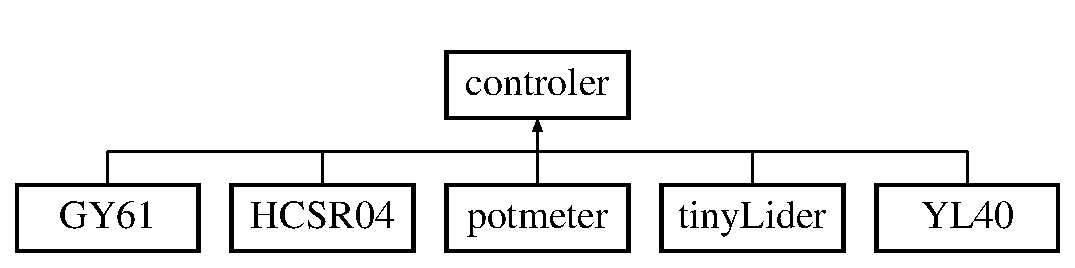
\includegraphics[height=2.000000cm]{classcontroler}
\end{center}
\end{figure}
\subsection*{Public Member Functions}
\begin{DoxyCompactItemize}
\item 
\mbox{\hyperlink{classcontroler_a9c52c62aa5a072b7853d711f3337f11b}{controler}} ()
\begin{DoxyCompactList}\small\item\em controller \end{DoxyCompactList}\item 
\mbox{\Hypertarget{classcontroler_a3c8e3c641d371c50a53780d104a3c016}\label{classcontroler_a3c8e3c641d371c50a53780d104a3c016}} 
virtual int {\bfseries get} ()=0
\end{DoxyCompactItemize}


\subsection{Constructor \& Destructor Documentation}
\mbox{\Hypertarget{classcontroler_a9c52c62aa5a072b7853d711f3337f11b}\label{classcontroler_a9c52c62aa5a072b7853d711f3337f11b}} 
\index{controler@{controler}!controler@{controler}}
\index{controler@{controler}!controler@{controler}}
\subsubsection{\texorpdfstring{controler()}{controler()}}
{\footnotesize\ttfamily controler\+::controler (\begin{DoxyParamCaption}{ }\end{DoxyParamCaption})}



controller 

\begin{DoxyAuthor}{Author}
Thomas Theil 
\end{DoxyAuthor}
\begin{DoxyDate}{Date}
25-\/06-\/2018 14\+:00
\end{DoxyDate}
Abstract controler class 

The documentation for this class was generated from the following files\+:\begin{DoxyCompactItemize}
\item 
controler.\+hpp\item 
controler.\+cpp\end{DoxyCompactItemize}

\hypertarget{classc_paddel}{}\section{c\+Paddel Class Reference}
\label{classc_paddel}\index{c\+Paddel@{c\+Paddel}}
\subsection*{Public Member Functions}
\begin{DoxyCompactItemize}
\item 
\mbox{\hyperlink{classc_paddel_ac907920de815a71e07e129e511f13db4}{c\+Paddel}} (int posX, int posY, \mbox{\hyperlink{classcontroler}{controler}} \&inputcontroler)
\begin{DoxyCompactList}\small\item\em \mbox{\hyperlink{classc_paddel_ac907920de815a71e07e129e511f13db4}{c\+Paddel(int pos\+X, int pos\+Y, controler \& inputcontroler)}}. \end{DoxyCompactList}\item 
void \mbox{\hyperlink{classc_paddel_a4bdcfa64ad3713e749574894d45a8d3b}{Reset}} ()
\begin{DoxyCompactList}\small\item\em \mbox{\hyperlink{classc_paddel_a4bdcfa64ad3713e749574894d45a8d3b}{Reset()}} \end{DoxyCompactList}\item 
int \mbox{\hyperlink{classc_paddel_aaa833a367eab3cc275d7b67b4c3b68e4}{getX}} ()
\begin{DoxyCompactList}\small\item\em \mbox{\hyperlink{classc_paddel_aaa833a367eab3cc275d7b67b4c3b68e4}{get\+X()}} \end{DoxyCompactList}\item 
int \mbox{\hyperlink{classc_paddel_a96cd3a3c7f5678b7e5f8f4eaca271ba2}{getY}} ()
\begin{DoxyCompactList}\small\item\em \mbox{\hyperlink{classc_paddel_a96cd3a3c7f5678b7e5f8f4eaca271ba2}{get\+Y()}} \end{DoxyCompactList}\item 
char \mbox{\hyperlink{classc_paddel_ab291cc9d81b3d169d11fba7d7b57186d}{paddel\+Size}} (char new\+Size=0)
\begin{DoxyCompactList}\small\item\em \mbox{\hyperlink{classc_paddel_ab291cc9d81b3d169d11fba7d7b57186d}{paddel\+Size(char new\+Size)}} \end{DoxyCompactList}\item 
void \mbox{\hyperlink{classc_paddel_a0ef466b341239bf42708ec3e64e942b5}{update}} ()
\begin{DoxyCompactList}\small\item\em \mbox{\hyperlink{classc_paddel_a0ef466b341239bf42708ec3e64e942b5}{update()}} \end{DoxyCompactList}\end{DoxyCompactItemize}


\subsection{Constructor \& Destructor Documentation}
\mbox{\Hypertarget{classc_paddel_ac907920de815a71e07e129e511f13db4}\label{classc_paddel_ac907920de815a71e07e129e511f13db4}} 
\index{c\+Paddel@{c\+Paddel}!c\+Paddel@{c\+Paddel}}
\index{c\+Paddel@{c\+Paddel}!c\+Paddel@{c\+Paddel}}
\subsubsection{\texorpdfstring{c\+Paddel()}{cPaddel()}}
{\footnotesize\ttfamily c\+Paddel\+::c\+Paddel (\begin{DoxyParamCaption}\item[{int}]{posX,  }\item[{int}]{posY,  }\item[{\mbox{\hyperlink{classcontroler}{controler}} \&}]{inputcontroler }\end{DoxyParamCaption})}



\mbox{\hyperlink{classc_paddel_ac907920de815a71e07e129e511f13db4}{c\+Paddel(int pos\+X, int pos\+Y, controler \& inputcontroler)}}. 

\begin{DoxyAuthor}{Author}
Thomas Theil 
\end{DoxyAuthor}
\begin{DoxyDate}{Date}
25-\/06-\/2018 20\+:30
\end{DoxyDate}
The main controler class for the peddels

\begin{DoxyPrecond}{Precondition}
This class needs a controler input for it to work 
\end{DoxyPrecond}
\mbox{\hyperlink{classc_paddel}{c\+Paddel}} initialize(exampel) 
\begin{DoxyCode}
 \mbox{\hyperlink{class_h_c_s_r04}{HCSR04}} controler1();
\mbox{\hyperlink{classc_paddel}{cPaddel}} player1(X,Y,controler1);
\end{DoxyCode}
 

\subsection{Member Function Documentation}
\mbox{\Hypertarget{classc_paddel_aaa833a367eab3cc275d7b67b4c3b68e4}\label{classc_paddel_aaa833a367eab3cc275d7b67b4c3b68e4}} 
\index{c\+Paddel@{c\+Paddel}!getX@{getX}}
\index{getX@{getX}!c\+Paddel@{c\+Paddel}}
\subsubsection{\texorpdfstring{get\+X()}{getX()}}
{\footnotesize\ttfamily int c\+Paddel\+::getX (\begin{DoxyParamCaption}{ }\end{DoxyParamCaption})}



\mbox{\hyperlink{classc_paddel_aaa833a367eab3cc275d7b67b4c3b68e4}{get\+X()}} 

Get the X axis \begin{DoxyReturn}{Returns}
int 
\end{DoxyReturn}
\mbox{\Hypertarget{classc_paddel_a96cd3a3c7f5678b7e5f8f4eaca271ba2}\label{classc_paddel_a96cd3a3c7f5678b7e5f8f4eaca271ba2}} 
\index{c\+Paddel@{c\+Paddel}!getY@{getY}}
\index{getY@{getY}!c\+Paddel@{c\+Paddel}}
\subsubsection{\texorpdfstring{get\+Y()}{getY()}}
{\footnotesize\ttfamily int c\+Paddel\+::getY (\begin{DoxyParamCaption}{ }\end{DoxyParamCaption})}



\mbox{\hyperlink{classc_paddel_a96cd3a3c7f5678b7e5f8f4eaca271ba2}{get\+Y()}} 

Get the Y axis \begin{DoxyReturn}{Returns}
int 
\end{DoxyReturn}
\mbox{\Hypertarget{classc_paddel_ab291cc9d81b3d169d11fba7d7b57186d}\label{classc_paddel_ab291cc9d81b3d169d11fba7d7b57186d}} 
\index{c\+Paddel@{c\+Paddel}!paddel\+Size@{paddel\+Size}}
\index{paddel\+Size@{paddel\+Size}!c\+Paddel@{c\+Paddel}}
\subsubsection{\texorpdfstring{paddel\+Size()}{paddelSize()}}
{\footnotesize\ttfamily char c\+Paddel\+::paddel\+Size (\begin{DoxyParamCaption}\item[{char}]{new\+Size = {\ttfamily 0} }\end{DoxyParamCaption})}



\mbox{\hyperlink{classc_paddel_ab291cc9d81b3d169d11fba7d7b57186d}{paddel\+Size(char new\+Size)}} 

You can give the paddel a new\+Size. if you leef the new\+Size empty it wil be seen as a 0 ~\newline
it will return the new size of the paddel \begin{DoxyReturn}{Returns}
char 
\end{DoxyReturn}
\mbox{\Hypertarget{classc_paddel_a4bdcfa64ad3713e749574894d45a8d3b}\label{classc_paddel_a4bdcfa64ad3713e749574894d45a8d3b}} 
\index{c\+Paddel@{c\+Paddel}!Reset@{Reset}}
\index{Reset@{Reset}!c\+Paddel@{c\+Paddel}}
\subsubsection{\texorpdfstring{Reset()}{Reset()}}
{\footnotesize\ttfamily void c\+Paddel\+::\+Reset (\begin{DoxyParamCaption}{ }\end{DoxyParamCaption})}



\mbox{\hyperlink{classc_paddel_a4bdcfa64ad3713e749574894d45a8d3b}{Reset()}} 

Resets the paddels to its originals starting position \mbox{\Hypertarget{classc_paddel_a0ef466b341239bf42708ec3e64e942b5}\label{classc_paddel_a0ef466b341239bf42708ec3e64e942b5}} 
\index{c\+Paddel@{c\+Paddel}!update@{update}}
\index{update@{update}!c\+Paddel@{c\+Paddel}}
\subsubsection{\texorpdfstring{update()}{update()}}
{\footnotesize\ttfamily void c\+Paddel\+::update (\begin{DoxyParamCaption}{ }\end{DoxyParamCaption})}



\mbox{\hyperlink{classc_paddel_a0ef466b341239bf42708ec3e64e942b5}{update()}} 

update the position of the paddel on a screen of 64px height 

The documentation for this class was generated from the following files\+:\begin{DoxyCompactItemize}
\item 
c\+Paddel.\+hpp\item 
c\+Paddel.\+cpp\end{DoxyCompactItemize}

\hypertarget{class_g_y61}{}\section{G\+Y61 Class Reference}
\label{class_g_y61}\index{G\+Y61@{G\+Y61}}
Inheritance diagram for G\+Y61\+:\begin{figure}[H]
\begin{center}
\leavevmode
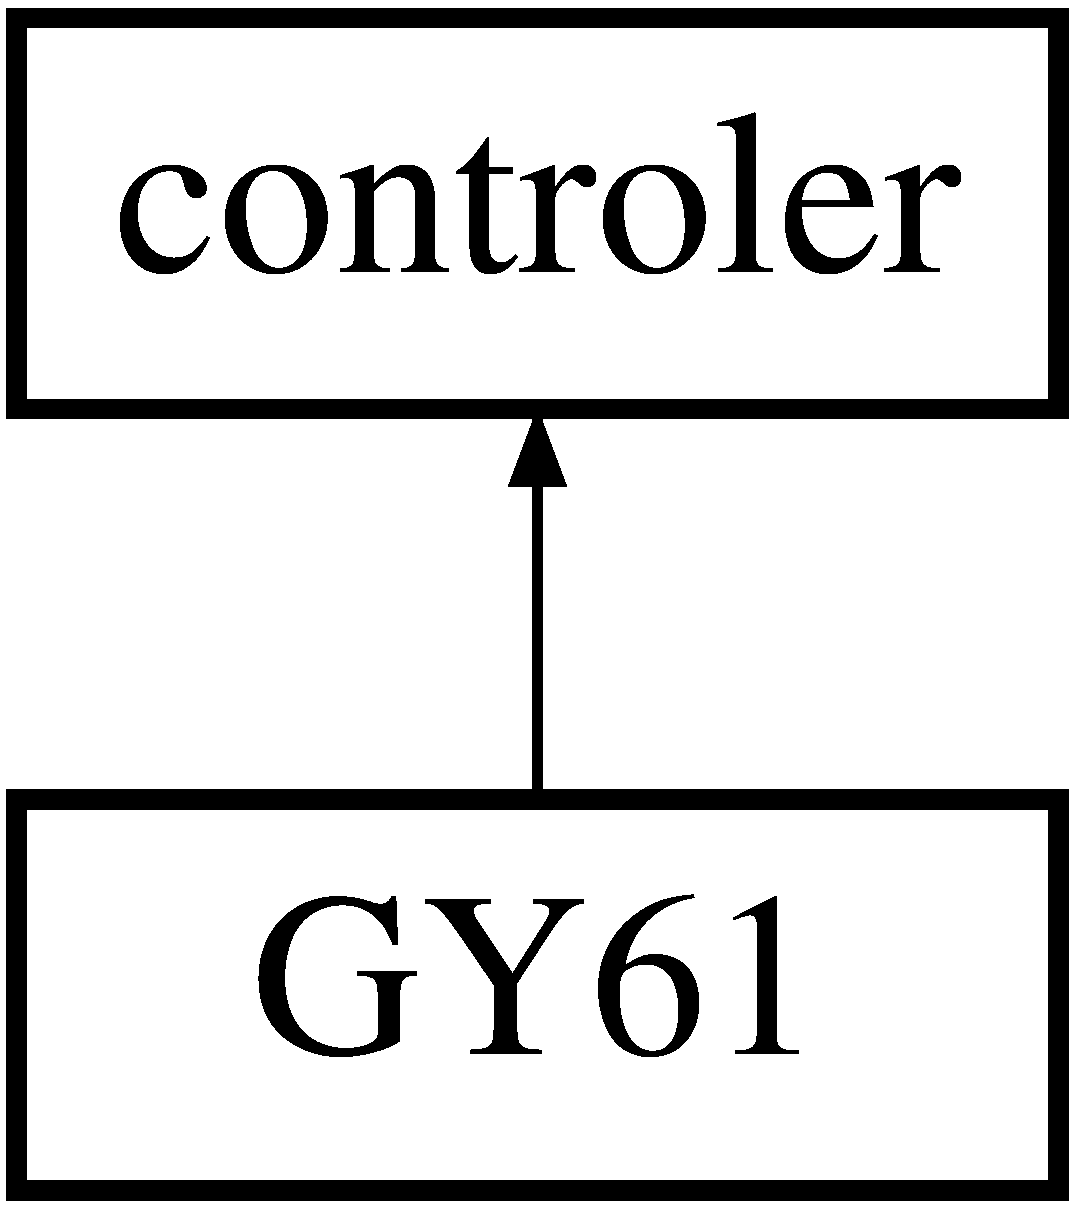
\includegraphics[height=2.000000cm]{class_g_y61}
\end{center}
\end{figure}
\subsection*{Public Member Functions}
\begin{DoxyCompactItemize}
\item 
\mbox{\hyperlink{class_g_y61_a2599179d0c2c4c26e87aab76ab6ee410}{G\+Y61}} (\mbox{\hyperlink{class_y_l40}{Y\+L40}} \&A\+D\+Ci2, char axis)
\begin{DoxyCompactList}\small\item\em G\+Y-\/61 chip. \end{DoxyCompactList}\item 
int \mbox{\hyperlink{class_g_y61_a3163809be7dd33dc0c46ba503b55394a}{get}} ()
\begin{DoxyCompactList}\small\item\em \mbox{\hyperlink{class_g_y61_a3163809be7dd33dc0c46ba503b55394a}{get()}} \end{DoxyCompactList}\end{DoxyCompactItemize}
\subsection*{Public Attributes}
\begin{DoxyCompactItemize}
\item 
\mbox{\Hypertarget{class_g_y61_a40d6e29cc3b8a0701689f868cc82ee1f}\label{class_g_y61_a40d6e29cc3b8a0701689f868cc82ee1f}} 
\mbox{\hyperlink{class_y_l40}{Y\+L40}} \& {\bfseries A\+D\+Ci2}
\item 
\mbox{\Hypertarget{class_g_y61_a0f96ea841bdcf07771c613bf16be6bb9}\label{class_g_y61_a0f96ea841bdcf07771c613bf16be6bb9}} 
char {\bfseries axis} = 0
\item 
\mbox{\Hypertarget{class_g_y61_adc2d00c3ffff2985240cad4808422e0b}\label{class_g_y61_adc2d00c3ffff2985240cad4808422e0b}} 
int {\bfseries base}
\end{DoxyCompactItemize}


\subsection{Constructor \& Destructor Documentation}
\mbox{\Hypertarget{class_g_y61_a2599179d0c2c4c26e87aab76ab6ee410}\label{class_g_y61_a2599179d0c2c4c26e87aab76ab6ee410}} 
\index{G\+Y61@{G\+Y61}!G\+Y61@{G\+Y61}}
\index{G\+Y61@{G\+Y61}!G\+Y61@{G\+Y61}}
\subsubsection{\texorpdfstring{G\+Y61()}{GY61()}}
{\footnotesize\ttfamily G\+Y61\+::\+G\+Y61 (\begin{DoxyParamCaption}\item[{\mbox{\hyperlink{class_y_l40}{Y\+L40}} \&}]{A\+D\+Ci2,  }\item[{char}]{axis }\end{DoxyParamCaption})}



G\+Y-\/61 chip. 

\begin{DoxyAuthor}{Author}
Thomas Theil 
\end{DoxyAuthor}
\begin{DoxyDate}{Date}
26-\/06-\/2018 15\+:00
\end{DoxyDate}
read out the G\+Y-\/61 chip using tha Y\+L-\/40 for more information loop at \mbox{\hyperlink{class_y_l40}{Y\+L40()}}

\begin{DoxyPrecond}{Precondition}
This class uses \mbox{\hyperlink{class_y_l40}{Y\+L40}} for its workings 
\end{DoxyPrecond}
potmeter initialize(exampel) 
\begin{DoxyCode}
\textcolor{keyword}{auto} scl     = target::pin\_oc( target::pins::scl );
\textcolor{keyword}{auto} sda      = target::pin\_oc( target::pins::sda );
\textcolor{keyword}{auto} i2c\_bus = hwlib::i2c\_bus\_bit\_banged\_scl\_sda( scl, sda );
\mbox{\hyperlink{class_y_l40}{YL40}} ADCi2(i2c\_bus, 0x48);
\mbox{\hyperlink{class_g_y61}{GY61}} controler2(ADCi2);
\end{DoxyCode}


\begin{DoxyWarning}{Warning}
This class needs hwlib and \mbox{\hyperlink{class_y_l40}{Y\+L40}} to work. 
\end{DoxyWarning}


\subsection{Member Function Documentation}
\mbox{\Hypertarget{class_g_y61_a3163809be7dd33dc0c46ba503b55394a}\label{class_g_y61_a3163809be7dd33dc0c46ba503b55394a}} 
\index{G\+Y61@{G\+Y61}!get@{get}}
\index{get@{get}!G\+Y61@{G\+Y61}}
\subsubsection{\texorpdfstring{get()}{get()}}
{\footnotesize\ttfamily int G\+Y61\+::get (\begin{DoxyParamCaption}{ }\end{DoxyParamCaption})\hspace{0.3cm}{\ttfamily [virtual]}}



\mbox{\hyperlink{class_g_y61_a3163809be7dd33dc0c46ba503b55394a}{get()}} 

Get the output of the A/D

returns int 

Implements \mbox{\hyperlink{classcontroler}{controler}}.



The documentation for this class was generated from the following files\+:\begin{DoxyCompactItemize}
\item 
G\+Y61.\+hpp\item 
G\+Y61.\+cpp\end{DoxyCompactItemize}

\hypertarget{class_h_c_s_r04}{}\section{H\+C\+S\+R04 Class Reference}
\label{class_h_c_s_r04}\index{H\+C\+S\+R04@{H\+C\+S\+R04}}
Inheritance diagram for H\+C\+S\+R04\+:\begin{figure}[H]
\begin{center}
\leavevmode
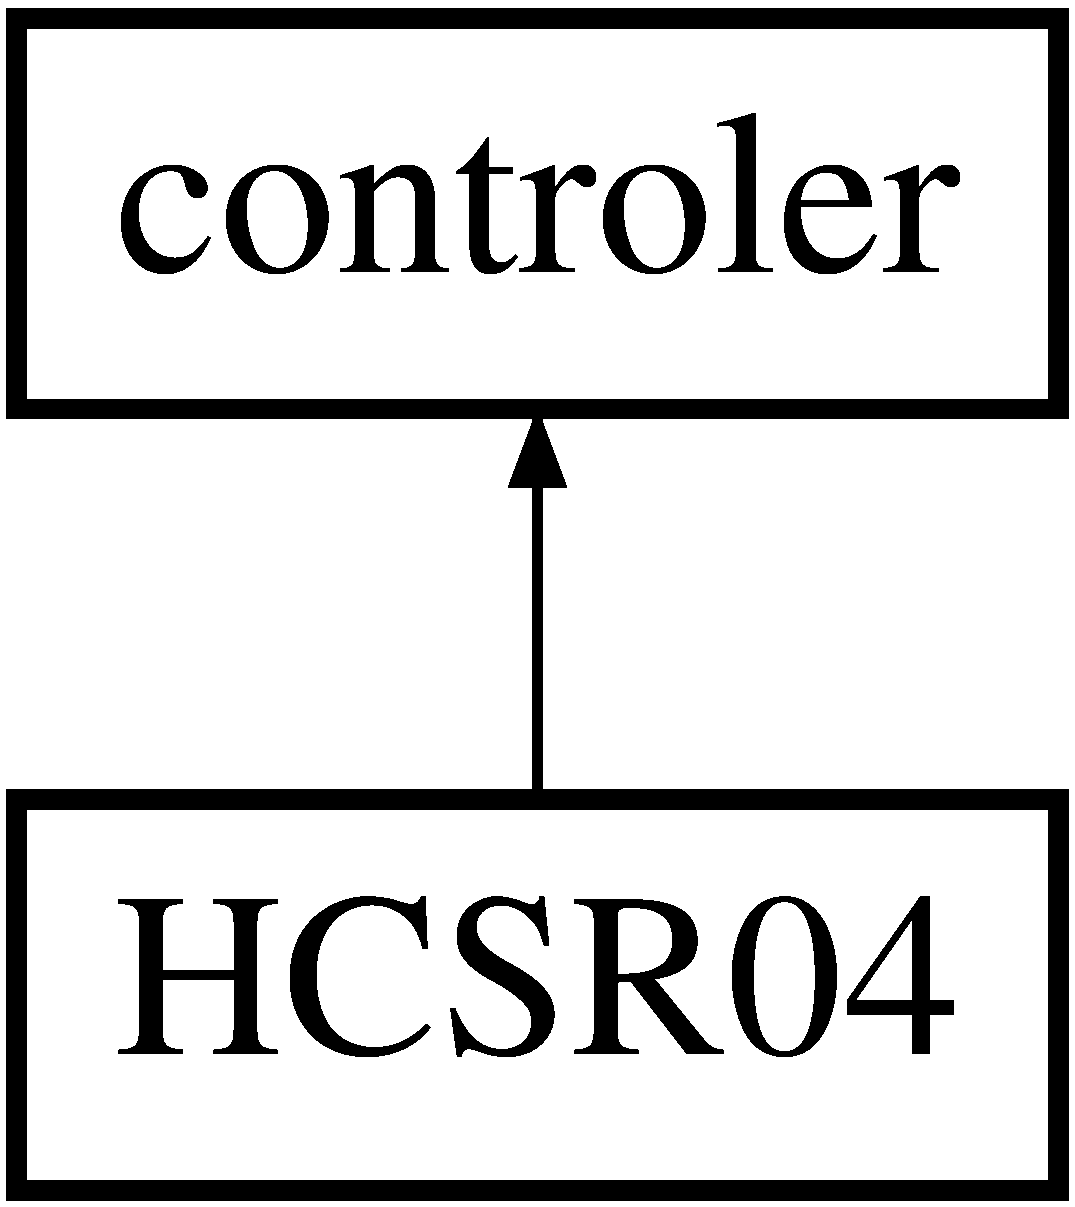
\includegraphics[height=2.000000cm]{class_h_c_s_r04}
\end{center}
\end{figure}
\subsection*{Public Member Functions}
\begin{DoxyCompactItemize}
\item 
\mbox{\hyperlink{class_h_c_s_r04_a6630d5354ee9fb0abdb70c5dbbb2e130}{H\+C\+S\+R04}} (hwlib\+::target\+::pin\+\_\+out \&trigger, hwlib\+::target\+::pin\+\_\+in \&echo)
\begin{DoxyCompactList}\small\item\em \mbox{\hyperlink{class_h_c_s_r04}{H\+C\+S\+R04}} sensor class. \end{DoxyCompactList}\item 
int \mbox{\hyperlink{class_h_c_s_r04_aced49671ccc6cf679e045d2fb9709d8c}{get}} ()
\begin{DoxyCompactList}\small\item\em Get() \end{DoxyCompactList}\end{DoxyCompactItemize}


\subsection{Constructor \& Destructor Documentation}
\mbox{\Hypertarget{class_h_c_s_r04_a6630d5354ee9fb0abdb70c5dbbb2e130}\label{class_h_c_s_r04_a6630d5354ee9fb0abdb70c5dbbb2e130}} 
\index{H\+C\+S\+R04@{H\+C\+S\+R04}!H\+C\+S\+R04@{H\+C\+S\+R04}}
\index{H\+C\+S\+R04@{H\+C\+S\+R04}!H\+C\+S\+R04@{H\+C\+S\+R04}}
\subsubsection{\texorpdfstring{H\+C\+S\+R04()}{HCSR04()}}
{\footnotesize\ttfamily H\+C\+S\+R04\+::\+H\+C\+S\+R04 (\begin{DoxyParamCaption}\item[{hwlib\+::target\+::pin\+\_\+out \&}]{trigger,  }\item[{hwlib\+::target\+::pin\+\_\+in \&}]{echo }\end{DoxyParamCaption})}



\mbox{\hyperlink{class_h_c_s_r04}{H\+C\+S\+R04}} sensor class. 

\begin{DoxyAuthor}{Author}
Thomas Theil 
\end{DoxyAuthor}
\begin{DoxyDate}{Date}
25-\/06-\/2018 14\+:00
\end{DoxyDate}
This class wil read out the H\+C-\/\+S\+R04 Ultrasonic Sensor.~\newline
 \begin{DoxyPrecond}{Precondition}
To construct this class will need one output pin and one inputpin !. 
\end{DoxyPrecond}
\mbox{\hyperlink{class_h_c_s_r04}{H\+C\+S\+R04}} initialize(exampel) 
\begin{DoxyCode}
\textcolor{keyword}{auto} trigger = target::pin\_out(target::pins::d7);
\textcolor{keyword}{auto} echo    = target::pin\_in(target::pins::d6);
\mbox{\hyperlink{class_h_c_s_r04}{HCSR04}} sensor2(trigger,echo);
\end{DoxyCode}


\begin{DoxyWarning}{Warning}
This class needs hwlib to work. 
\end{DoxyWarning}


\subsection{Member Function Documentation}
\mbox{\Hypertarget{class_h_c_s_r04_aced49671ccc6cf679e045d2fb9709d8c}\label{class_h_c_s_r04_aced49671ccc6cf679e045d2fb9709d8c}} 
\index{H\+C\+S\+R04@{H\+C\+S\+R04}!get@{get}}
\index{get@{get}!H\+C\+S\+R04@{H\+C\+S\+R04}}
\subsubsection{\texorpdfstring{get()}{get()}}
{\footnotesize\ttfamily int H\+C\+S\+R04\+::get (\begin{DoxyParamCaption}{ }\end{DoxyParamCaption})\hspace{0.3cm}{\ttfamily [virtual]}}



Get() 

Getting the distance that calculate of the H\+C-\/\+S\+R04 The distance is in \% calculate of the max distance 150.

\begin{DoxyWarning}{Warning}
The bigger the distance is the slower the function will response
\end{DoxyWarning}
\begin{DoxyReturn}{Returns}
int ~\newline
 \mbox{\hyperlink{class_h_c_s_r04_aced49671ccc6cf679e045d2fb9709d8c}{H\+C\+S\+R04.\+get()}}
\end{DoxyReturn}
\begin{DoxyParagraph}{example}

\begin{DoxyCode}
sensor2.get();
\end{DoxyCode}
 
\end{DoxyParagraph}


Implements \mbox{\hyperlink{classcontroler}{controler}}.



The documentation for this class was generated from the following files\+:\begin{DoxyCompactItemize}
\item 
H\+C\+S\+R04.\+hpp\item 
H\+C\+S\+R04.\+cpp\end{DoxyCompactItemize}

\hypertarget{classpiezo}{}\section{piezo Class Reference}
\label{classpiezo}\index{piezo@{piezo}}
\subsection*{Public Member Functions}
\begin{DoxyCompactItemize}
\item 
\mbox{\hyperlink{classpiezo_aa7daa7fd80b5580bd2c5e379a69ffdc4}{piezo}} (hwlib\+::target\+::pin\+\_\+out \&output)
\begin{DoxyCompactList}\small\item\em Piezo buzzer class. \end{DoxyCompactList}\item 
void \mbox{\hyperlink{classpiezo_ac14361f4fb7fe063b8c4455946220ee4}{tone}} (unsigned int tone, int duration)
\begin{DoxyCompactList}\small\item\em Tone. \end{DoxyCompactList}\item 
void \mbox{\hyperlink{classpiezo_a4e92d8bc5b101f9862a089134518c55f}{song}} (int notes\mbox{[}$\,$\mbox{]}, int duration\mbox{[}$\,$\mbox{]}, int lenght)
\begin{DoxyCompactList}\small\item\em song \end{DoxyCompactList}\end{DoxyCompactItemize}


\subsection{Constructor \& Destructor Documentation}
\mbox{\Hypertarget{classpiezo_aa7daa7fd80b5580bd2c5e379a69ffdc4}\label{classpiezo_aa7daa7fd80b5580bd2c5e379a69ffdc4}} 
\index{piezo@{piezo}!piezo@{piezo}}
\index{piezo@{piezo}!piezo@{piezo}}
\subsubsection{\texorpdfstring{piezo()}{piezo()}}
{\footnotesize\ttfamily piezo\+::piezo (\begin{DoxyParamCaption}\item[{hwlib\+::target\+::pin\+\_\+out \&}]{output }\end{DoxyParamCaption})}



Piezo buzzer class. 

\begin{DoxyAuthor}{Author}
Thomas Theil 
\end{DoxyAuthor}
\begin{DoxyDate}{Date}
25-\/06-\/2018 15\+:30
\end{DoxyDate}
This class wil output a sound over a piezo buzzer. ~\newline
 \begin{DoxyPrecond}{Precondition}
To construct this class will need a output pin. 
\end{DoxyPrecond}
Piezo initialize 
\begin{DoxyCode}
\textcolor{keyword}{auto} buzzerPin  = target::pin\_out(target::pins::d5);
\mbox{\hyperlink{classpiezo}{piezo}} buzzer(buzzerPin);
\end{DoxyCode}


\begin{DoxyWarning}{Warning}
This class requers hwlib to work. 
\end{DoxyWarning}


\subsection{Member Function Documentation}
\mbox{\Hypertarget{classpiezo_a4e92d8bc5b101f9862a089134518c55f}\label{classpiezo_a4e92d8bc5b101f9862a089134518c55f}} 
\index{piezo@{piezo}!song@{song}}
\index{song@{song}!piezo@{piezo}}
\subsubsection{\texorpdfstring{song()}{song()}}
{\footnotesize\ttfamily void piezo\+::song (\begin{DoxyParamCaption}\item[{int}]{notes\mbox{[}$\,$\mbox{]},  }\item[{int}]{duration\mbox{[}$\,$\mbox{]},  }\item[{int}]{lenght }\end{DoxyParamCaption})}



song 

will play the song you made juses \mbox{\hyperlink{classpiezo_ac14361f4fb7fe063b8c4455946220ee4}{tone()}} as base


\begin{DoxyParams}{Parameters}
{\em int} & notes\mbox{[}\mbox{]} (Array of all the notes that will be played) ~\newline
 input can be your own note or one of the Preloaded \mbox{\hyperlink{classpiezo_ac14361f4fb7fe063b8c4455946220ee4}{tone()}}. \\
\hline
{\em int} & duration \mbox{[}\mbox{]} (Array of all the lenghs that the notes will play for) \\
\hline
{\em int} & lenght (The lenght of the input arrays)\\
\hline
\end{DoxyParams}
\begin{DoxyParagraph}{example}

\begin{DoxyCode}
\textcolor{keywordtype}{char}  notes[8]  = \{\textcolor{charliteral}{'c'},\textcolor{charliteral}{'d'},\textcolor{charliteral}{'e'},\textcolor{charliteral}{'f'},\textcolor{charliteral}{'g'},\textcolor{charliteral}{'a'},\textcolor{charliteral}{'b'},\textcolor{charliteral}{'C'}\};
\textcolor{keywordtype}{int}  lenght[8] = \{300,300,300,300,300,300,300,300\};
buzzer.song(notes,lenght,8);
\end{DoxyCode}
 
\end{DoxyParagraph}
\begin{DoxyReturn}{Returns}
void 
\end{DoxyReturn}
\mbox{\Hypertarget{classpiezo_ac14361f4fb7fe063b8c4455946220ee4}\label{classpiezo_ac14361f4fb7fe063b8c4455946220ee4}} 
\index{piezo@{piezo}!tone@{tone}}
\index{tone@{tone}!piezo@{piezo}}
\subsubsection{\texorpdfstring{tone()}{tone()}}
{\footnotesize\ttfamily void piezo\+::tone (\begin{DoxyParamCaption}\item[{unsigned int}]{tone,  }\item[{int}]{duration }\end{DoxyParamCaption})}



Tone. 

It will ouput a tone over the piezo buzzer.


\begin{DoxyParams}{Parameters}
{\em char} & tone (The tone that will be will sound) ~\newline
 input can be your own note or one of the Preloaded \\
\hline
{\em int} & duration (The miliseconds the tone will sound for)\\
\hline
\end{DoxyParams}
\begin{DoxyParagraph}{Preloaded notes}
{\bfseries c} 262\+Hz ~\newline
 {\bfseries d} 294\+Hz ~\newline
 {\bfseries e} 330\+Hz ~\newline
 {\bfseries f} 349\+Hz ~\newline
 {\bfseries g} 392\+Hz ~\newline
 {\bfseries a} 440\+Hz ~\newline
 {\bfseries b} 494\+Hz ~\newline
 {\bfseries C} 523\+Hz ~\newline
 
\end{DoxyParagraph}
\begin{DoxyWarning}{Warning}
duration of 0 stil result in a sound
\end{DoxyWarning}
\begin{DoxyParagraph}{example}

\begin{DoxyCode}
buzzer.tone(\textcolor{charliteral}{'a'},1000);
\end{DoxyCode}
 
\end{DoxyParagraph}
\begin{DoxyReturn}{Returns}
void 
\end{DoxyReturn}


The documentation for this class was generated from the following files\+:\begin{DoxyCompactItemize}
\item 
piezo.\+hpp\item 
piezo.\+cpp\end{DoxyCompactItemize}

\hypertarget{classpong_manger}{}\section{pong\+Manger Class Reference}
\label{classpong_manger}\index{pong\+Manger@{pong\+Manger}}
\subsection*{Public Member Functions}
\begin{DoxyCompactItemize}
\item 
\mbox{\hyperlink{classpong_manger_a757b4d3c1ace0490604e4f93da6b5a04}{pong\+Manger}} (hwlib\+::glcd\+\_\+oled \&oled, \mbox{\hyperlink{classc_ball}{c\+Ball}} \&ball, \mbox{\hyperlink{classc_paddel}{c\+Paddel}} \&player1, \mbox{\hyperlink{classc_paddel}{c\+Paddel}} \&player2, \mbox{\hyperlink{classpiezo}{piezo}} \&sound)
\begin{DoxyCompactList}\small\item\em \mbox{\hyperlink{classpong_manger_a757b4d3c1ace0490604e4f93da6b5a04}{pong\+Manger(hwlib\+::glcd\+\_\+oled  \& oled, c\+Ball \& ball, c\+Paddel \& player1, c\+Paddel \& player2, piezo \& sound)}}. \end{DoxyCompactList}\item 
void \mbox{\hyperlink{classpong_manger_a2c2c6e7f024261d5b3e3f4b85abb060a}{Draw}} ()
\begin{DoxyCompactList}\small\item\em \mbox{\hyperlink{classpong_manger_a2c2c6e7f024261d5b3e3f4b85abb060a}{Draw()}} \end{DoxyCompactList}\item 
void \mbox{\hyperlink{classpong_manger_a878b50d69f98eb0de013269fbf9b0ead}{Update}} ()
\begin{DoxyCompactList}\small\item\em \mbox{\hyperlink{classpong_manger_a878b50d69f98eb0de013269fbf9b0ead}{Update()}} \end{DoxyCompactList}\item 
void \mbox{\hyperlink{classpong_manger_a177da6a9f5120dc153b8f33d8e6bebc3}{collision}} ()
\begin{DoxyCompactList}\small\item\em \mbox{\hyperlink{classpong_manger_a177da6a9f5120dc153b8f33d8e6bebc3}{collision()}} \end{DoxyCompactList}\end{DoxyCompactItemize}


\subsection{Constructor \& Destructor Documentation}
\mbox{\Hypertarget{classpong_manger_a757b4d3c1ace0490604e4f93da6b5a04}\label{classpong_manger_a757b4d3c1ace0490604e4f93da6b5a04}} 
\index{pong\+Manger@{pong\+Manger}!pong\+Manger@{pong\+Manger}}
\index{pong\+Manger@{pong\+Manger}!pong\+Manger@{pong\+Manger}}
\subsubsection{\texorpdfstring{pong\+Manger()}{pongManger()}}
{\footnotesize\ttfamily pong\+Manger\+::pong\+Manger (\begin{DoxyParamCaption}\item[{hwlib\+::glcd\+\_\+oled \&}]{oled,  }\item[{\mbox{\hyperlink{classc_ball}{c\+Ball}} \&}]{ball,  }\item[{\mbox{\hyperlink{classc_paddel}{c\+Paddel}} \&}]{player1,  }\item[{\mbox{\hyperlink{classc_paddel}{c\+Paddel}} \&}]{player2,  }\item[{\mbox{\hyperlink{classpiezo}{piezo}} \&}]{sound }\end{DoxyParamCaption})}



\mbox{\hyperlink{classpong_manger_a757b4d3c1ace0490604e4f93da6b5a04}{pong\+Manger(hwlib\+::glcd\+\_\+oled  \& oled, c\+Ball \& ball, c\+Paddel \& player1, c\+Paddel \& player2, piezo \& sound)}}. 

\begin{DoxyAuthor}{Author}
Thomas Theil 
\end{DoxyAuthor}
\begin{DoxyDate}{Date}
25-\/06-\/2018 21\+:30
\end{DoxyDate}
The pong game class ~\newline
The class wil controle the pong game

\begin{DoxyPrecond}{Precondition}
hwlib a must to run this 
\end{DoxyPrecond}
\mbox{\hyperlink{classpong_manger}{pong\+Manger(exampel)}} 
\begin{DoxyCode}
\mbox{\hyperlink{classc_ball}{cBall}} ball(64,32);
\mbox{\hyperlink{classc_paddel}{cPaddel}} player1(1,0,controler1);
\mbox{\hyperlink{classc_paddel}{cPaddel}} player2(127,0,controler1);

\mbox{\hyperlink{classpong_manger}{pongManger}} pong(oled,ball,player1,player2,buzzer);
\textcolor{keywordflow}{while}(1)\{
    pong.Update();
    pong.Draw();

\}
\end{DoxyCode}
 

\subsection{Member Function Documentation}
\mbox{\Hypertarget{classpong_manger_a177da6a9f5120dc153b8f33d8e6bebc3}\label{classpong_manger_a177da6a9f5120dc153b8f33d8e6bebc3}} 
\index{pong\+Manger@{pong\+Manger}!collision@{collision}}
\index{collision@{collision}!pong\+Manger@{pong\+Manger}}
\subsubsection{\texorpdfstring{collision()}{collision()}}
{\footnotesize\ttfamily void pong\+Manger\+::collision (\begin{DoxyParamCaption}{ }\end{DoxyParamCaption})}



\mbox{\hyperlink{classpong_manger_a177da6a9f5120dc153b8f33d8e6bebc3}{collision()}} 

This function will check if there hase been any colission with the object. ~\newline
when a collision is detected a sound wil play out of the piezo speaker ~\newline
~\newline
if the bal reaches one side the game wil end and a sound will play~\newline
the game will restart on its own \mbox{\Hypertarget{classpong_manger_a2c2c6e7f024261d5b3e3f4b85abb060a}\label{classpong_manger_a2c2c6e7f024261d5b3e3f4b85abb060a}} 
\index{pong\+Manger@{pong\+Manger}!Draw@{Draw}}
\index{Draw@{Draw}!pong\+Manger@{pong\+Manger}}
\subsubsection{\texorpdfstring{Draw()}{Draw()}}
{\footnotesize\ttfamily void pong\+Manger\+::\+Draw (\begin{DoxyParamCaption}{ }\end{DoxyParamCaption})}



\mbox{\hyperlink{classpong_manger_a2c2c6e7f024261d5b3e3f4b85abb060a}{Draw()}} 

Will draw to the conected oled screen \mbox{\Hypertarget{classpong_manger_a878b50d69f98eb0de013269fbf9b0ead}\label{classpong_manger_a878b50d69f98eb0de013269fbf9b0ead}} 
\index{pong\+Manger@{pong\+Manger}!Update@{Update}}
\index{Update@{Update}!pong\+Manger@{pong\+Manger}}
\subsubsection{\texorpdfstring{Update()}{Update()}}
{\footnotesize\ttfamily void pong\+Manger\+::\+Update (\begin{DoxyParamCaption}{ }\end{DoxyParamCaption})}



\mbox{\hyperlink{classpong_manger_a878b50d69f98eb0de013269fbf9b0ead}{Update()}} 

Update\textquotesingle{}s the position of all the objects. ~\newline
It wil also run a \mbox{\hyperlink{classpong_manger_a177da6a9f5120dc153b8f33d8e6bebc3}{collision()}} 

The documentation for this class was generated from the following files\+:\begin{DoxyCompactItemize}
\item 
pong\+Manger.\+hpp\item 
pong\+Manger.\+cpp\end{DoxyCompactItemize}

\hypertarget{classpotmeter}{}\section{potmeter Class Reference}
\label{classpotmeter}\index{potmeter@{potmeter}}
Inheritance diagram for potmeter\+:\begin{figure}[H]
\begin{center}
\leavevmode
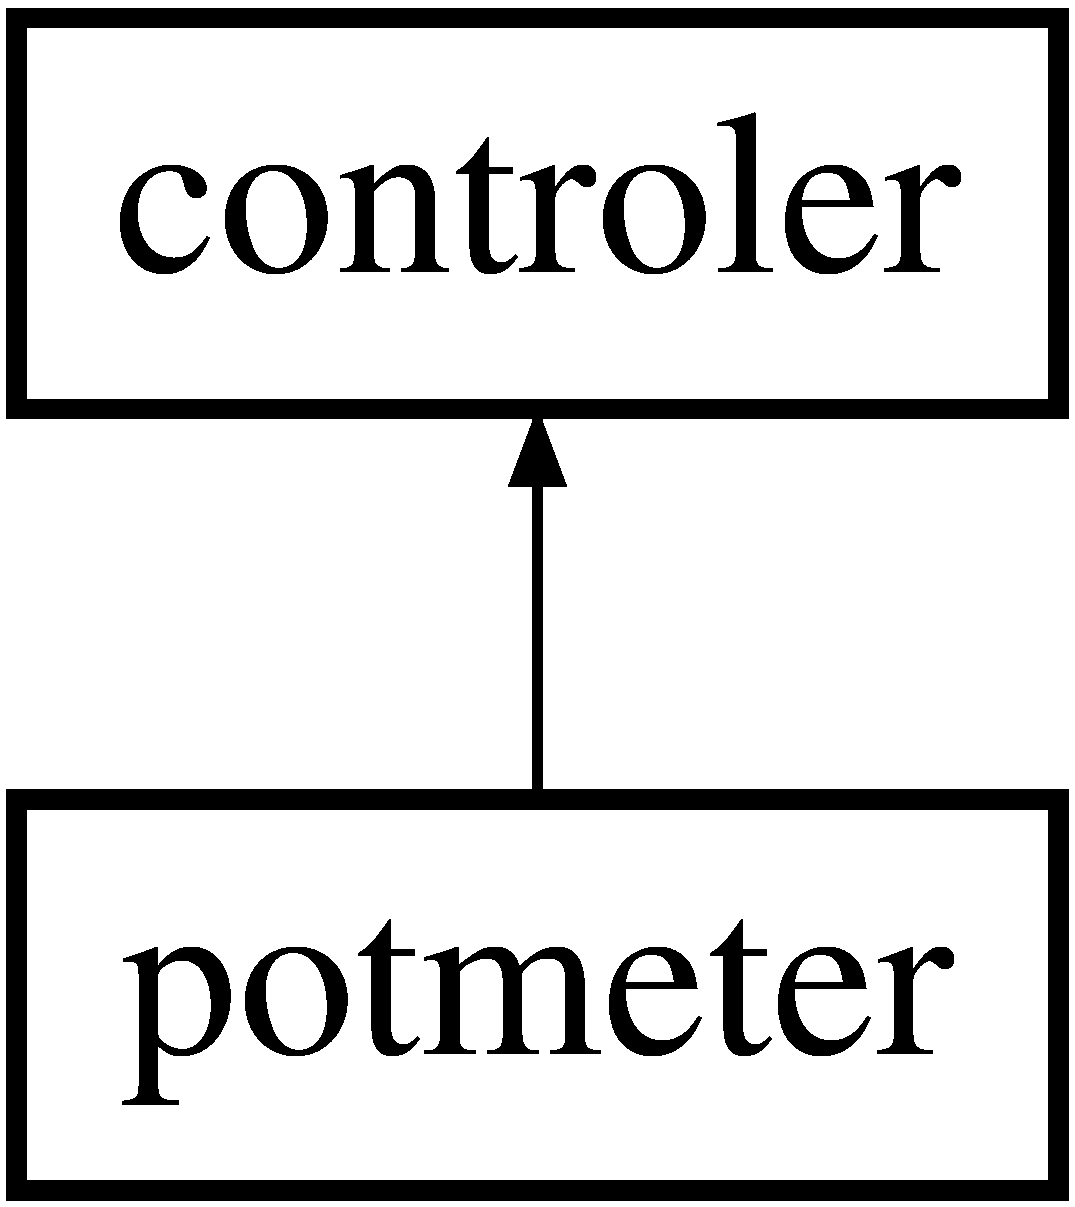
\includegraphics[height=2.000000cm]{classpotmeter}
\end{center}
\end{figure}
\subsection*{Public Member Functions}
\begin{DoxyCompactItemize}
\item 
\mbox{\hyperlink{classpotmeter_a30949c70814bb0cd26d8bb043529ce59}{potmeter}} (\mbox{\hyperlink{class_y_l40}{Y\+L40}} \&A\+D\+Ci2)
\begin{DoxyCompactList}\small\item\em potmeter readout \end{DoxyCompactList}\item 
int \mbox{\hyperlink{classpotmeter_a9184480674fac846504a03a77036dd71}{get}} ()
\begin{DoxyCompactList}\small\item\em \mbox{\hyperlink{classpotmeter_a9184480674fac846504a03a77036dd71}{get()}} \end{DoxyCompactList}\end{DoxyCompactItemize}
\subsection*{Public Attributes}
\begin{DoxyCompactItemize}
\item 
\mbox{\Hypertarget{classpotmeter_af61db45fd919db8beabc841c800d3e1c}\label{classpotmeter_af61db45fd919db8beabc841c800d3e1c}} 
\mbox{\hyperlink{class_y_l40}{Y\+L40}} \& {\bfseries A\+D\+Ci2}
\end{DoxyCompactItemize}


\subsection{Constructor \& Destructor Documentation}
\mbox{\Hypertarget{classpotmeter_a30949c70814bb0cd26d8bb043529ce59}\label{classpotmeter_a30949c70814bb0cd26d8bb043529ce59}} 
\index{potmeter@{potmeter}!potmeter@{potmeter}}
\index{potmeter@{potmeter}!potmeter@{potmeter}}
\subsubsection{\texorpdfstring{potmeter()}{potmeter()}}
{\footnotesize\ttfamily potmeter\+::potmeter (\begin{DoxyParamCaption}\item[{\mbox{\hyperlink{class_y_l40}{Y\+L40}} \&}]{A\+D\+Ci2 }\end{DoxyParamCaption})}



potmeter readout 

\begin{DoxyAuthor}{Author}
Thomas Theil 
\end{DoxyAuthor}
\begin{DoxyDate}{Date}
26-\/06-\/2018 14\+:30
\end{DoxyDate}
read out the potmeter using tha \mbox{\hyperlink{class_y_l40}{Y\+L40}} for more information loop at \mbox{\hyperlink{class_y_l40}{Y\+L40()}}

\begin{DoxyPrecond}{Precondition}
This class uses \mbox{\hyperlink{class_y_l40}{Y\+L40}} for its workings 
\end{DoxyPrecond}
potmeter initialize(exampel) 
\begin{DoxyCode}
\textcolor{keyword}{auto} scl     = target::pin\_oc( target::pins::scl );
\textcolor{keyword}{auto} sda      = target::pin\_oc( target::pins::sda );
\textcolor{keyword}{auto} i2c\_bus = hwlib::i2c\_bus\_bit\_banged\_scl\_sda( scl, sda );
\mbox{\hyperlink{class_y_l40}{YL40}} ADCi2(i2c\_bus, 0x48);
\mbox{\hyperlink{classpotmeter}{potmeter}} controler2(ADCi2);
\end{DoxyCode}


\begin{DoxyWarning}{Warning}
This class needs hwlib and \mbox{\hyperlink{class_y_l40}{Y\+L40}} to work. 
\end{DoxyWarning}


\subsection{Member Function Documentation}
\mbox{\Hypertarget{classpotmeter_a9184480674fac846504a03a77036dd71}\label{classpotmeter_a9184480674fac846504a03a77036dd71}} 
\index{potmeter@{potmeter}!get@{get}}
\index{get@{get}!potmeter@{potmeter}}
\subsubsection{\texorpdfstring{get()}{get()}}
{\footnotesize\ttfamily int potmeter\+::get (\begin{DoxyParamCaption}{ }\end{DoxyParamCaption})\hspace{0.3cm}{\ttfamily [virtual]}}



\mbox{\hyperlink{classpotmeter_a9184480674fac846504a03a77036dd71}{get()}} 

Get the output of the A/D

returns int 

Implements \mbox{\hyperlink{classcontroler}{controler}}.



The documentation for this class was generated from the following files\+:\begin{DoxyCompactItemize}
\item 
potmeter.\+hpp\item 
potmeter.\+cpp\end{DoxyCompactItemize}

\hypertarget{classtiny_lider}{}\section{tiny\+Lider Class Reference}
\label{classtiny_lider}\index{tiny\+Lider@{tiny\+Lider}}
Inheritance diagram for tiny\+Lider\+:\begin{figure}[H]
\begin{center}
\leavevmode
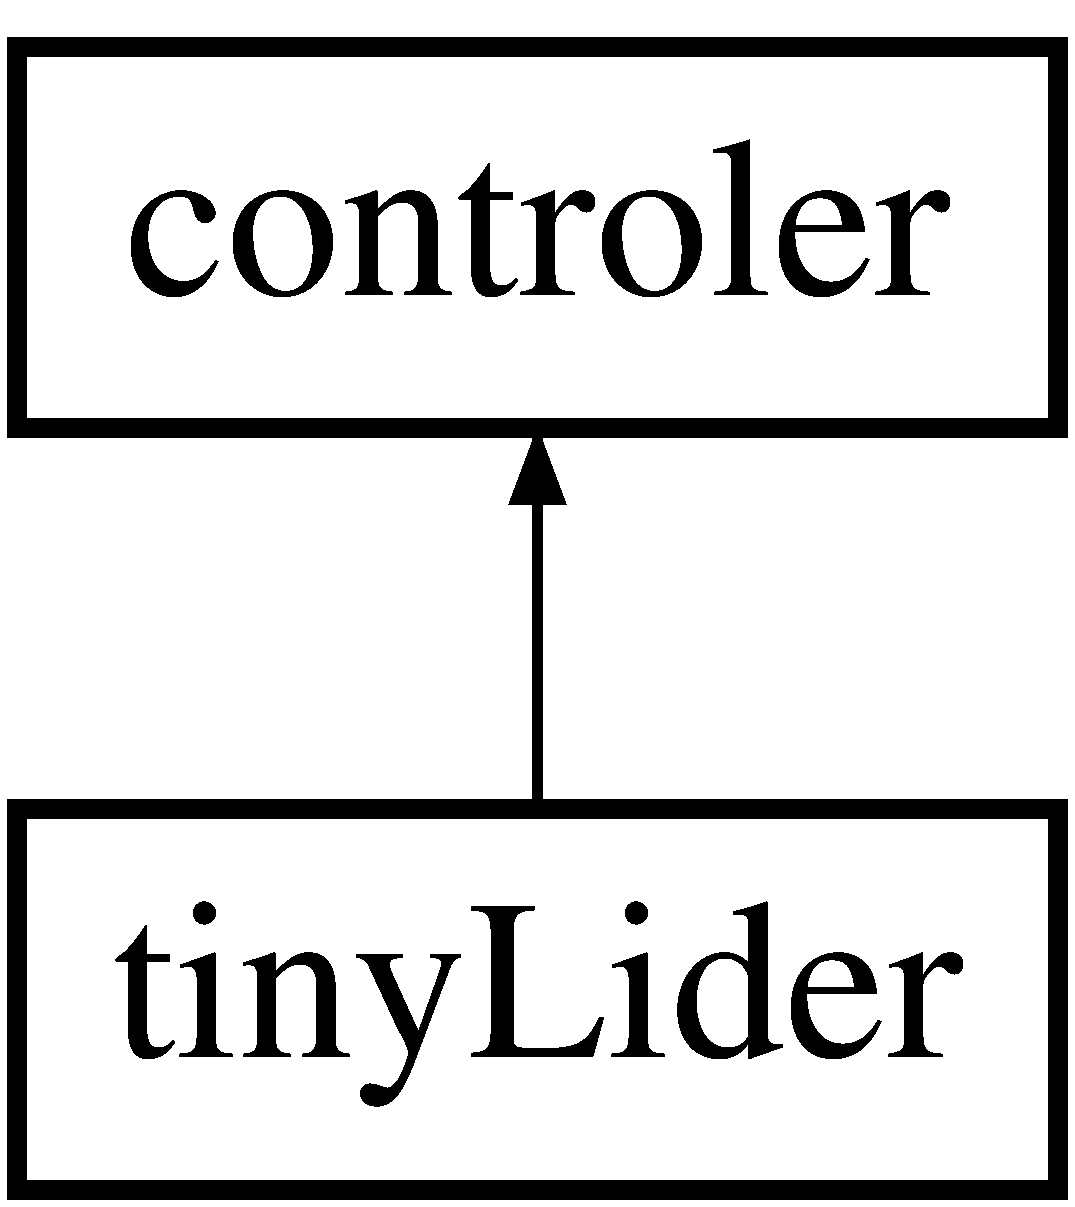
\includegraphics[height=2.000000cm]{classtiny_lider}
\end{center}
\end{figure}
\subsection*{Public Member Functions}
\begin{DoxyCompactItemize}
\item 
\mbox{\hyperlink{classtiny_lider_a68b7cd779d6cec28f53a3c4f4c858c11}{tiny\+Lider}} (char slave, hwlib\+::i2c\+\_\+bus\+\_\+bit\+\_\+banged\+\_\+scl\+\_\+sda \&i2c\+\_\+bus)
\begin{DoxyCompactList}\small\item\em \mbox{\hyperlink{classtiny_lider}{tiny\+Lider}} \end{DoxyCompactList}\item 
int \mbox{\hyperlink{classtiny_lider_ac69b92b0bd4056f6378e7e13aafa57b5}{get}} ()
\begin{DoxyCompactList}\small\item\em \mbox{\hyperlink{classtiny_lider_ac69b92b0bd4056f6378e7e13aafa57b5}{get()}} \end{DoxyCompactList}\end{DoxyCompactItemize}


\subsection{Constructor \& Destructor Documentation}
\mbox{\Hypertarget{classtiny_lider_a68b7cd779d6cec28f53a3c4f4c858c11}\label{classtiny_lider_a68b7cd779d6cec28f53a3c4f4c858c11}} 
\index{tiny\+Lider@{tiny\+Lider}!tiny\+Lider@{tiny\+Lider}}
\index{tiny\+Lider@{tiny\+Lider}!tiny\+Lider@{tiny\+Lider}}
\subsubsection{\texorpdfstring{tiny\+Lider()}{tinyLider()}}
{\footnotesize\ttfamily tiny\+Lider\+::tiny\+Lider (\begin{DoxyParamCaption}\item[{char}]{slave,  }\item[{hwlib\+::i2c\+\_\+bus\+\_\+bit\+\_\+banged\+\_\+scl\+\_\+sda \&}]{i2c\+\_\+bus }\end{DoxyParamCaption})}



\mbox{\hyperlink{classtiny_lider}{tiny\+Lider}} 

\begin{DoxyAuthor}{Author}
Thomas Theil 
\end{DoxyAuthor}
\begin{DoxyDate}{Date}
24-\/06-\/2018 16\+:00
\end{DoxyDate}
This class will read out the tiny\+Lidar module

\begin{DoxyPrecond}{Precondition}
It needs i2c to read the tinylidar 
\end{DoxyPrecond}
\begin{DoxyParagraph}{i2c adress}
the i2c adress is 0x10. for more information go to \href{https://microedco.s3.amazonaws.com/tinyLiDAR/Documentation/tinyLiDAR%20Reference%20Manual%20rev1.26.pdf}{\tt tiny\+Lidar}
\end{DoxyParagraph}
\mbox{\hyperlink{classtiny_lider}{tiny\+Lider}} initialize(example) 
\begin{DoxyCode}
\textcolor{keyword}{auto} scl     = target::pin\_oc( target::pins::scl );
\textcolor{keyword}{auto} sda      = target::pin\_oc( target::pins::sda );
\textcolor{keyword}{auto} i2c\_bus = hwlib::i2c\_bus\_bit\_banged\_scl\_sda( scl, sda );
tinylidar sensor1 (0x10 ,i2c\_bus);
\end{DoxyCode}


\begin{DoxyWarning}{Warning}
This class needs hwlib to work. 
\end{DoxyWarning}


\subsection{Member Function Documentation}
\mbox{\Hypertarget{classtiny_lider_ac69b92b0bd4056f6378e7e13aafa57b5}\label{classtiny_lider_ac69b92b0bd4056f6378e7e13aafa57b5}} 
\index{tiny\+Lider@{tiny\+Lider}!get@{get}}
\index{get@{get}!tiny\+Lider@{tiny\+Lider}}
\subsubsection{\texorpdfstring{get()}{get()}}
{\footnotesize\ttfamily int tiny\+Lider\+::get (\begin{DoxyParamCaption}{ }\end{DoxyParamCaption})\hspace{0.3cm}{\ttfamily [virtual]}}



\mbox{\hyperlink{classtiny_lider_ac69b92b0bd4056f6378e7e13aafa57b5}{get()}} 

Get the distance in MM of the tiny\+Lidar

\begin{DoxyParagraph}{Workings}
The class will get a average of 3 readings.
\end{DoxyParagraph}
\mbox{\hyperlink{classtiny_lider}{tiny\+Lider}} initialize(example) 
\begin{DoxyCode}
\mbox{\hyperlink{classtiny_lider}{tinyLider}}.\mbox{\hyperlink{classtiny_lider_ac69b92b0bd4056f6378e7e13aafa57b5}{get}}();
\end{DoxyCode}


\begin{DoxyReturn}{Returns}
int 
\end{DoxyReturn}


Implements \mbox{\hyperlink{classcontroler}{controler}}.



The documentation for this class was generated from the following files\+:\begin{DoxyCompactItemize}
\item 
tiny\+Lidar.\+hpp\item 
tiny\+Lidar.\+cpp\end{DoxyCompactItemize}

\hypertarget{class_y_l40}{}\section{Y\+L40 Class Reference}
\label{class_y_l40}\index{Y\+L40@{Y\+L40}}
Inheritance diagram for Y\+L40\+:\begin{figure}[H]
\begin{center}
\leavevmode
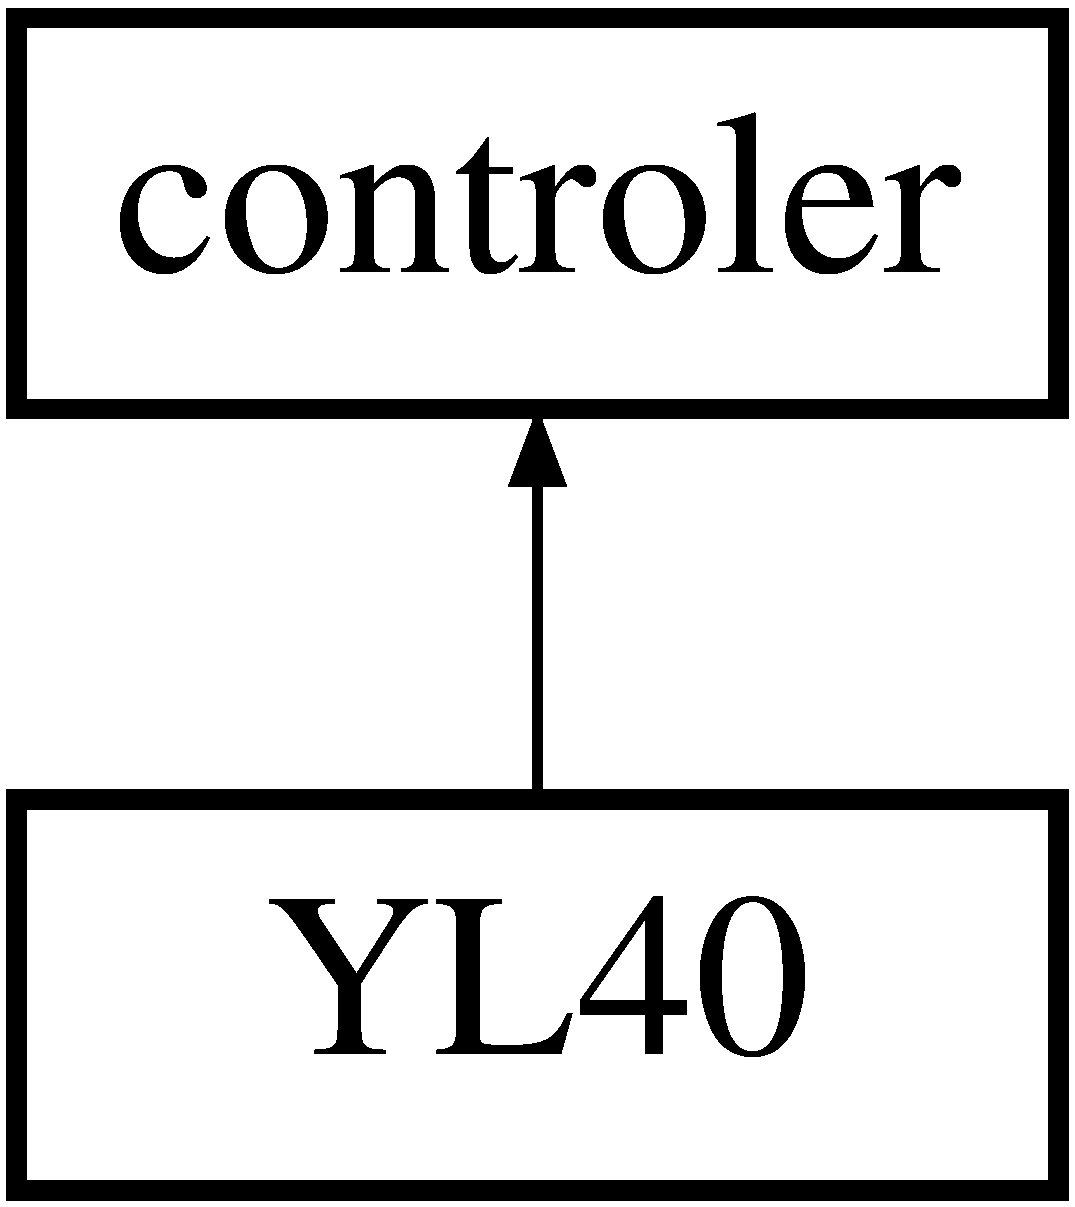
\includegraphics[height=2.000000cm]{class_y_l40}
\end{center}
\end{figure}
\subsection*{Public Member Functions}
\begin{DoxyCompactItemize}
\item 
\mbox{\hyperlink{class_y_l40_a5cbc98cfd60b1d4fd489dfa79254fd33}{Y\+L40}} (hwlib\+::i2c\+\_\+bus\+\_\+bit\+\_\+banged\+\_\+scl\+\_\+sda \&i2c\+\_\+bus, char slave)
\begin{DoxyCompactList}\small\item\em Y\+L-\/40 A\+D\+C/\+D\+AC chip. \end{DoxyCompactList}\item 
int \mbox{\hyperlink{class_y_l40_a3e0322c2c8c8dfed7466056173bc563e}{get}} ()
\begin{DoxyCompactList}\small\item\em \mbox{\hyperlink{class_y_l40_a3e0322c2c8c8dfed7466056173bc563e}{get()}} \end{DoxyCompactList}\item 
void \mbox{\hyperlink{class_y_l40_a97593c0f3ab5284c2a1258ed81f32d96}{changreadout}} (char pin)
\begin{DoxyCompactList}\small\item\em changereadout(char pin) \end{DoxyCompactList}\item 
\mbox{\Hypertarget{class_y_l40_aec31472494c65121f87be43d9a12878e}\label{class_y_l40_aec31472494c65121f87be43d9a12878e}} 
void {\bfseries wirte} ()
\item 
\mbox{\Hypertarget{class_y_l40_a2f1f0be24016335020ff75ff36b5693f}\label{class_y_l40_a2f1f0be24016335020ff75ff36b5693f}} 
void {\bfseries singe\+Wave} (char wave\+Type, int duration)
\end{DoxyCompactItemize}


\subsection{Constructor \& Destructor Documentation}
\mbox{\Hypertarget{class_y_l40_a5cbc98cfd60b1d4fd489dfa79254fd33}\label{class_y_l40_a5cbc98cfd60b1d4fd489dfa79254fd33}} 
\index{Y\+L40@{Y\+L40}!Y\+L40@{Y\+L40}}
\index{Y\+L40@{Y\+L40}!Y\+L40@{Y\+L40}}
\subsubsection{\texorpdfstring{Y\+L40()}{YL40()}}
{\footnotesize\ttfamily Y\+L40\+::\+Y\+L40 (\begin{DoxyParamCaption}\item[{hwlib\+::i2c\+\_\+bus\+\_\+bit\+\_\+banged\+\_\+scl\+\_\+sda \&}]{i2c\+\_\+bus,  }\item[{char}]{slave }\end{DoxyParamCaption})}



Y\+L-\/40 A\+D\+C/\+D\+AC chip. 

\begin{DoxyAuthor}{Author}
Thomas Theil 
\end{DoxyAuthor}
\begin{DoxyDate}{Date}
26-\/06-\/2018 14\+:00
\end{DoxyDate}
This class controles the Y\+L-\/40 board using the P\+C\+F8591 chip. ~\newline
The P\+C\+F891 chip is a A/D and D/A converter controled via I2C. ~\newline
for the data sheet folow \href{https://www.aurel32.net/elec/pcf8591.pdf}{\tt This} link. After boot the chip wil auto read Analog in 0

\begin{DoxyParagraph}{i2c adress}
the i2c adress is 0x48.
\end{DoxyParagraph}
\begin{DoxyPrecond}{Precondition}
This chips needs a hwlib i2c to work 
\end{DoxyPrecond}
Y\+L-\/40 initialize(exampel) 
\begin{DoxyCode}
\textcolor{keyword}{auto} scl     = target::pin\_oc( target::pins::scl );
\textcolor{keyword}{auto} sda      = target::pin\_oc( target::pins::sda );
\textcolor{keyword}{auto} i2c\_bus = hwlib::i2c\_bus\_bit\_banged\_scl\_sda( scl, sda );
\mbox{\hyperlink{class_y_l40}{YL40}} ADCi2(i2c\_bus, 0x48);
\end{DoxyCode}


\begin{DoxyWarning}{Warning}
This class needs hwlib to work. 
\end{DoxyWarning}


\subsection{Member Function Documentation}
\mbox{\Hypertarget{class_y_l40_a97593c0f3ab5284c2a1258ed81f32d96}\label{class_y_l40_a97593c0f3ab5284c2a1258ed81f32d96}} 
\index{Y\+L40@{Y\+L40}!changreadout@{changreadout}}
\index{changreadout@{changreadout}!Y\+L40@{Y\+L40}}
\subsubsection{\texorpdfstring{changreadout()}{changreadout()}}
{\footnotesize\ttfamily void Y\+L40\+::changreadout (\begin{DoxyParamCaption}\item[{char}]{pin }\end{DoxyParamCaption})}



changereadout(char pin) 

This function changes the read out pin of the chip

\begin{DoxyParagraph}{Pins}
{\bfseries A\+I\+N0} 0 ~\newline
 {\bfseries A\+I\+N1} 1 ~\newline
 {\bfseries A\+I\+N2} 2 ~\newline
 {\bfseries A\+I\+N3} 3 ~\newline

\end{DoxyParagraph}
\mbox{\Hypertarget{class_y_l40_a3e0322c2c8c8dfed7466056173bc563e}\label{class_y_l40_a3e0322c2c8c8dfed7466056173bc563e}} 
\index{Y\+L40@{Y\+L40}!get@{get}}
\index{get@{get}!Y\+L40@{Y\+L40}}
\subsubsection{\texorpdfstring{get()}{get()}}
{\footnotesize\ttfamily int Y\+L40\+::get (\begin{DoxyParamCaption}{ }\end{DoxyParamCaption})\hspace{0.3cm}{\ttfamily [virtual]}}



\mbox{\hyperlink{class_y_l40_a3e0322c2c8c8dfed7466056173bc563e}{get()}} 

Get the output of the A/D

returns int 

Implements \mbox{\hyperlink{classcontroler}{controler}}.



The documentation for this class was generated from the following files\+:\begin{DoxyCompactItemize}
\item 
Y\+L40.\+hpp\item 
Y\+L40.\+cpp\end{DoxyCompactItemize}

%--- End generated contents ---

% Index
\backmatter
\newpage
\phantomsection
\clearemptydoublepage
\addcontentsline{toc}{chapter}{Index}
\printindex

\end{document}
